
\chapter{Algorithms and Branches\label{chpt:algorithms-and-branches}}

As discussed in section \ref{chpt:mdft}, in code MDFT, we evaluate
the functional $\mathcal{F}[\varphi]$ and its gradient $\delta\mathcal{F}[\varphi]/\delta\varphi$
in each iteration. Figure \ref{fig:find-eq-den} shows a detailed
portion of the total MDFT flow chart in figure \ref{fig:code-mdft},
including the functional evaluation and minimization.

\begin{figure}[h]
\begin{centering}
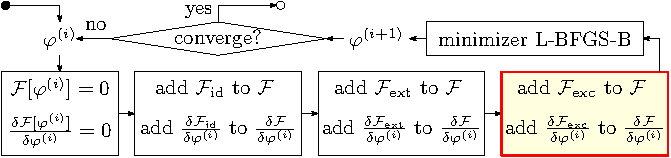
\includegraphics{_figure/find_equilibium_density}
\par\end{centering}
\caption[Process ``find equilibrium density'' in MDFT]{Process ``find equilibrium density'' in MDFT. After the ``initiation''
process, the flow chart begins at the black point. The three terms
of functional and their gradients are then accumulated in order. The
process ends at the white point, which then goes through the ``output''
process. \label{fig:find-eq-den}}
\end{figure}

As shown in figure \ref{fig:find-eq-den}, the three functional terms
and its gradients can be both calculated separately. With the first
two terms well presented in section \ref{chpt:mdft}, this section
aims to summary all the algorithms to evaluate the excess functional
gradient $\gamma(\mathbf{r},\mathbf{\Omega})$ from $\Delta\rho(\mathbf{r},\mathbf{\Omega})$,
knowing that
\begin{equation}
\rho(\mathbf{r},\mathbf{\Omega})=\rho_{0}\varphi^{2}(\mathbf{r},\mathbf{\Omega})
\end{equation}
\begin{equation}
\frac{\delta\mathcal{F}_{\mathrm{exc}}}{\delta\varphi}=-k_{\mathrm{B}}T\rho_{0}\varphi(\mathbf{r},\mathbf{\Omega})\gamma(\mathbf{r},\mathbf{\Omega})
\end{equation}
and the functional $\mathcal{F}_{\mathrm{exc}}$ can be calculated
as:
\begin{equation}
\mathcal{F}_{\mathrm{exc}}=-\frac{k_{\mathrm{B}}T}{2}\int\mathrm{d}\mathbf{r}\mathrm{d}\mathbf{\Omega}\Delta\rho(\mathbf{r},\mathbf{\Omega})\gamma(\mathbf{r},\mathbf{\Omega})
\end{equation}

According to the commutativity of operations (see $\mathsection$\ref{subsec:Commutativity-between-operations}),
the only possible algorithms to evaluate $\gamma(\mathbf{r},\mathbf{\Omega})$
from $\Delta\rho(\mathbf{r},\mathbf{\Omega})$ are shown in the figure
\ref{fig:Possible-algorithms}. We recall here that $\mathbf{\Omega}$
and $f_{\mu'\mu}^{m}$ refers to orientations in the laboratory frame
whereas $\boldsymbol{\omega}$ and ${f'}_{\chi\mu}^{m}$ refers to
orientations in the intermolecular frame (axis $\overrightarrow{Oz}$
in the direction of $\mathbf{k}$).

\begin{figure}[h]
\begin{centering}
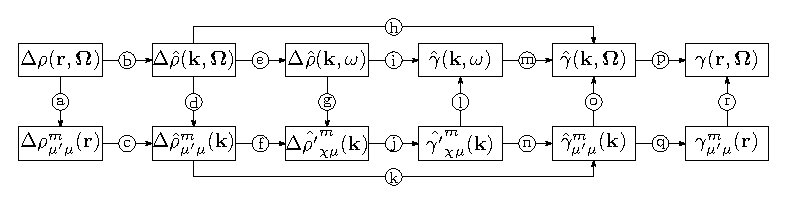
\includegraphics{_figure/algorithms}
\par\end{centering}
\caption{Possible algorithms for $\gamma$ evaluation\label{fig:Possible-algorithms}}
\end{figure}

Several branches are built to test and compare between algorithms,
which are shown below in table \ref{tab:Branch-option}. These branches
should give numerically the same result in certain conditions, that
will be discussed in later sections. 

\begin{table}[H]
\begin{centering}
\begin{tabular*}{1\textwidth}{@{\extracolsep{\fill}}cccc}
\toprule 
\tableheadline{Method} & \tableheadline{Sub-Method} & \tableheadline{Description} & \tableheadline{Theory}\tabularnewline
\midrule
reference & dipole & calculate $n(\mathbf{r})$ and $\mathbf{P}(\mathbf{r})$ separately & Ref \citep{Zhao_2011}\tabularnewline
\midrule
naive & standard & use $\hat{c}_{\mu\nu,\chi}^{mn}(k)$ as input \acs{DCF} & $\mathsection$\ref{subsec:Using-projections-in-1}\tabularnewline
 & zero-order & use $\hat{c}(k,\boldsymbol{\omega_{1}},\boldsymbol{\omega_{2}})$
and take the nearest point & $\mathsection$\ref{subsec:Zero-order-interpolation-of}\tabularnewline
 & interpolation & use $\hat{c}(k,\boldsymbol{\omega_{1}},\boldsymbol{\omega_{2}})$
with linear interpolation  & $\mathsection$\ref{subsec:Linear-interpolation-of}\tabularnewline
 & dipole & use $\hat{c}_{S}$, $\hat{c}_{\Delta}$, $\hat{c}_{D}$ issued from
\citep{zhao_accurate_2013} & $\mathsection$\ref{subsec:Using-projections-in}\tabularnewline
 & nmax1 & use $\hat{c}_{S}$, $\hat{c}_{\Delta}$, $\hat{c}_{D}$, $\hat{c}^{011}$
issued from \citep{puibasset_bridge_2012} & $\mathsection$\ref{subsec:Using-projections-in}\tabularnewline
\midrule
convolution & standard & algorithm with symmetry reduction & $\mathsection$\ref{subsec:Reduction-by-symmetry}\tabularnewline
 & asymm  & algorithm without symmetry reduction & $\mathsection$\ref{subsec:Reduction-by-symmetry}\tabularnewline
 & pure\_angular  & swap \acs{FFT} and \acs{FGSHT} & $\mathsection$\ref{chpt:algorithms-and-branches}\tabularnewline
\bottomrule
\end{tabular*}
\par\end{centering}
\caption{Branch option in MDFT\label{tab:Branch-option}}
\end{table}


\section{Branches ``naive''}

Branches \texttt{\textbf{naive}} are the algorithms mentioned in section
\ref{chpt:fft-spatial}, which go through the path 
\[
\left(b\right)\shortrightarrow\left(h\right)\shortrightarrow\left(p\right)
\]
in figure \ref{fig:Possible-algorithms}, calculating directly $\hat{\gamma}(\mathbf{k},\mathbf{\Omega})$
from $\Delta\hat{\rho}(\mathbf{k},\mathbf{\Omega})$ with
\begin{equation}
\hat{\gamma}(\mathbf{k},\mathbf{\Omega}_{1})=\int\mathrm{d}\mathbf{\Omega}_{2}\Delta\hat{\rho}(\mathbf{k},\mathbf{\Omega}_{2})\hat{c}(\mathbf{k},\mathbf{\Omega}_{1},\mathbf{\Omega}_{2})\label{eq:gamma-naive}
\end{equation}

The \acs{DCF} in laboratory frame, $\hat{c}(\mathbf{k},\mathbf{\Omega}_{1},\mathbf{\Omega}_{2})$,
is reconstructed from the intermolecular \acs{DCF}, $\hat{c}(k,\boldsymbol{\omega}_{1},\boldsymbol{\omega}_{2})$,
by a pre-established relation $\boldsymbol{\omega}(\mathbf{\Omega}_{1},\mathbf{\Omega}_{2})$.
The difference between branches is the way to calculate $\hat{c}(k,\boldsymbol{\omega}_{1},\boldsymbol{\omega}_{2})$.
Branch\textbf{ }\texttt{\textbf{naive\_standard}} use $c_{\mu\nu,\chi}^{mn}(k)$
as input \acs{DCF}, and calculate $\hat{c}(k,\boldsymbol{\omega}_{1},\boldsymbol{\omega}_{2})$
directly (eq. (\ref{eq:dcf-exact})) during the evaluation of eq.
(\ref{eq:gamma-naive}) with these coefficients. Branch \texttt{\textbf{naive\_zero-order}}
and \texttt{\textbf{naive\_interpolation}} use a pre-tabulated $\hat{c}(k,\boldsymbol{\omega}_{1},\boldsymbol{\omega}_{2})$
as input, either calculated from $c_{\mu\nu,\chi}^{mn}(k)$ or in
other way. Branch \texttt{\textbf{naive\_zero-order}} takes the neatest
point of $\hat{c}(k,\boldsymbol{\omega}_{1},\boldsymbol{\omega}_{2})$
according to the pre-established correspondence $\boldsymbol{\omega}(\mathbf{\Omega}_{1},\mathbf{\Omega}_{2})$,
while \texttt{\textbf{naive\_interpolation}} gives a linear interpolation
on $\boldsymbol{\omega}$. The former is rejected in the implementation
due to a lack of precision (appendix \ref{chpt:error-evaluation-interpolation-DCF}),
thus only\textbf{ }\texttt{\textbf{naive\_standard}} and \texttt{\textbf{naive\_interpolation}}
are practically in use, apart from the $n_{\max}=1$ cases discussed
later. For all \texttt{\textbf{naive}} methods, we always take the
nearest point of $\left\Vert \mathbf{k}\right\Vert $ in $c_{\mu\nu,\chi}^{mn}(k)$
or in $\hat{c}(k,\boldsymbol{\omega}_{1},\boldsymbol{\omega}_{2})$,
i.e. zeroth order interpolation for $k$.

It should be noted that although the intermolecular form of \acs{DCF}
(function or projections) is used in every branch \texttt{\textbf{naive}},
the \acs{DCF} in laboratory form $\hat{c}(\mathbf{k},\mathbf{\Omega}_{1},\mathbf{\Omega}_{2})$
needs to be calculated. To exactly take the path
\[
\left(b\right)\shortrightarrow\left(e\right)\shortrightarrow\left(i\right)\shortrightarrow\left(m\right)\shortrightarrow\left(p\right)
\]
with $(k,\boldsymbol{\omega}_{1},\boldsymbol{\omega}_{2})$ numbers
of \acs{FE} for \acs{OZ} equation, the density variable $\Delta\hat{\rho}(\mathbf{k},\mathbf{\Omega})$
should be interpolated on $\Delta\hat{\rho}(\mathbf{k},\boldsymbol{\omega})$,
which seems not to be a wise choice.

\section{Branches ``convolution''}

The method \texttt{\textbf{convolution}}, which are developed in the
objective of this thesis and detailed theoretically in section \ref{chpt:angular-convolution},
contains three branches.

Branches\textbf{ }\texttt{\textbf{convolution\_asymm}} and \texttt{\textbf{convolution\_standard}}
go through the path
\[
\left(a\right)\shortrightarrow\left(c\right)\shortrightarrow\left(f\right)\shortrightarrow\left(j\right)\shortrightarrow\left(n\right)\shortrightarrow\left(q\right)\shortrightarrow\left(r\right)
\]
with \texttt{\textbf{convolution\_asymm}} using the original algorithm
($\mathsection$\ref{sec:Operational-algorithm}) without symmetry
reduction ($\mathsection$\ref{subsec:Reduction-by-symmetry}), i.e.
artificially generating all the projections $\Delta\rho_{\mu'\mu}^{m}(\mathbf{r})$
from the projections of $\mu\geq0$ given implicitly by the real-to-complex
\acs{FGSHT} process; while \texttt{\textbf{convolution\_standard}}
takes only the projections $\mu\geq0$, calculate the projections
in local frame (eq. (\ref{eq:2.2.rho-rot-rho}))
\begin{equation}
\Delta\hat{\rho'}_{\chi\mu}^{m}(\mathbf{k})=\sum_{\mu'}\Delta\hat{\rho}_{\mu'\mu}^{m}(\mathbf{k})R_{\mu'\chi}^{m}(\mathbf{\hat{k}})
\end{equation}
 for all $\mu$ and $k_{3}\geq0$, with the symmetry relation (eq.
(\ref{eq:2.2.symm-rho-k}))
\begin{equation}
\Delta\hat{\rho}_{\mu'\mu}^{m}(\mathbf{k})=(-)^{\mu'+\mu}\Delta\hat{\rho}_{\underline{\mu'}\underline{\mu}}^{m*}(-\mathbf{k})
\end{equation}

Branch \texttt{\textbf{convolution\_pure\_angular}} goes through the
path 
\[
\left(b\right)\shortrightarrow\left(d\right)\shortrightarrow\left(f\right)\shortrightarrow\left(j\right)\shortrightarrow\left(n\right)\shortrightarrow\left(o\right)\shortrightarrow\left(p\right)
\]
which swaps the \acs{FFT} and \acs{FGSHT} processes. It takes implicitly
$k_{3}\geq0$ from the real-to-complex \acs{FFT} process, thus implements
the same number of \acs{FE} for the \acs{OZ} equation as \texttt{\textbf{convolution\_standard}}.

Theoretically, \texttt{\textbf{convolution\_standard}} should be the
fastest \texttt{\textbf{convolution}} method as its number of \acs{FE}
for \acs{FFT} process is depending on the number of projections $\Delta\rho_{\mu'\mu}^{m}$,
which is smaller than the number of \acs{FE} for \texttt{\textbf{convolution\_pure\_angular}}
depending on the number of angles $(\Theta,\Phi,\Psi)$.

\section{Testing branches for $n_{\max}=1$}

To show the mathematical equivalence between the branches, several
testing branches for $n_{\max}=1$ are built.

Branches \texttt{\textbf{naive\_dipole}} and \texttt{\textbf{naive\_nmax1}}
go through the path $\left(b\right)\shortrightarrow\left(h\right)\shortrightarrow\left(p\right)$,
calculating $\hat{c}(\mathbf{k},\mathbf{\Omega}_{1},\mathbf{\Omega}_{2})$
directly with the projections $\hat{c}^{mnl}(k)$ as shown in $\mathsection$\ref{subsec:Using-projections-in},
with separately the \acs{DCF} of the references \citep{zhao_accurate_2013}
and \citep{puibasset_bridge_2012}, whose slight difference is shown
in $\mathsection$\ref{subsec:Comparison-with-non-coupling}. 

Branch \texttt{\textbf{reference\_dipole}} use \acs{DCF} in \citep{zhao_accurate_2013},
which is the original method in \acs{MDFT} to calculate $\mathcal{F}_{\mathrm{exc}}$
via multipole expansion, and is mathematically equivalent to \texttt{\textbf{naive\_dipole}}.
In addition with branch \texttt{\textbf{convolution\_standard}} that
can also use the two \acs{DCF}s mentioned above, a test of validation
can be performed, which should in any case be exactly the same numerically
if the same \acs{DCF} is used.

\section{Other paths}

Considering the necessity, other paths such as those passing by $\left(k\right)$
are only built for local test usage (c.f. $\mathsection$\ref{subsec:A-single-k-kernel}
and $\mathsection$\ref{sec:-kernel}).
